\documentclass{article}

%------------------------------------------------------------------------------
%Packages
\usepackage{comment}
\usepackage[francais]{babel}
\usepackage[latin1]{inputenc}
\usepackage[T1]{fontenc}
\usepackage{graphicx}

%------------------------------------------------------------------------------

\title{Plee the Bear - Graphisme}
\author{Julien Jorge}
\date{\today}

\begin{document}

%------------------------------------------------------------------------------

\maketitle
\begin{abstract}
Ce document pr\'esente la fa\c con dont le jeu g\`ere les graphismes
et essaie d'expliquer quel niveau de qualit\'e visuelle nous voulons
atteindre. Nous ferons une pr\'esentation rapide de la structure des
niveaux, puis nous donnerons quelques d\'etails sur les restrictions
sur les sprites et, finalement, nous donnerons quelques r\`egles sur
la mani\`ere de faire de beaux dessins.
\end{abstract}

\tableofcontents
\newpage

%------------------------------------------------------------------------------
\section{Structure des niveaux}
Les niveaux sont faits avec plusieurs calques (voir
fig.~\ref{fig-layers-separated}). Du premier plan au dernier, nous
avons :
\begin{itemize}
\item un calque d'\'etat, avec les scores, les vies restantes, etc.
\item un calque de bulles, qui indique aussi la position des joueurs
      hors \'ecran ;
\item z\'ero ou plus calques de d\'ecoration, avec des sprites et des
      animations ;
\item un calque d'action, o\`u les joueurs et les ennemis sont ;
\item z\'ero ou plus calques de d\'ecoration.
\end{itemize}

La vue du joueur est repr\'esent\'ee par une cam\'era. Nous calculons
la vue courante par une projection orthogonale du contenu des calques
\`a travers le rectangle de la cam\'era (voir
fig.~\ref{fig-layers-result}). Nous utilisons le calque d'action comme
calque de r\'ef\'erence ; sa taille est exactement celle du
monde. Les calques les plus petits d\'efileront plus lentement, alors
que les plus grands d\'efileront plus rapidement. Par exemple, un
calque dont la taille est la moiti\'e de celle du calque d'action sur
chaque axe d\'efilera deux fois moins vite.

\begin{figure}
 \begin{center}
  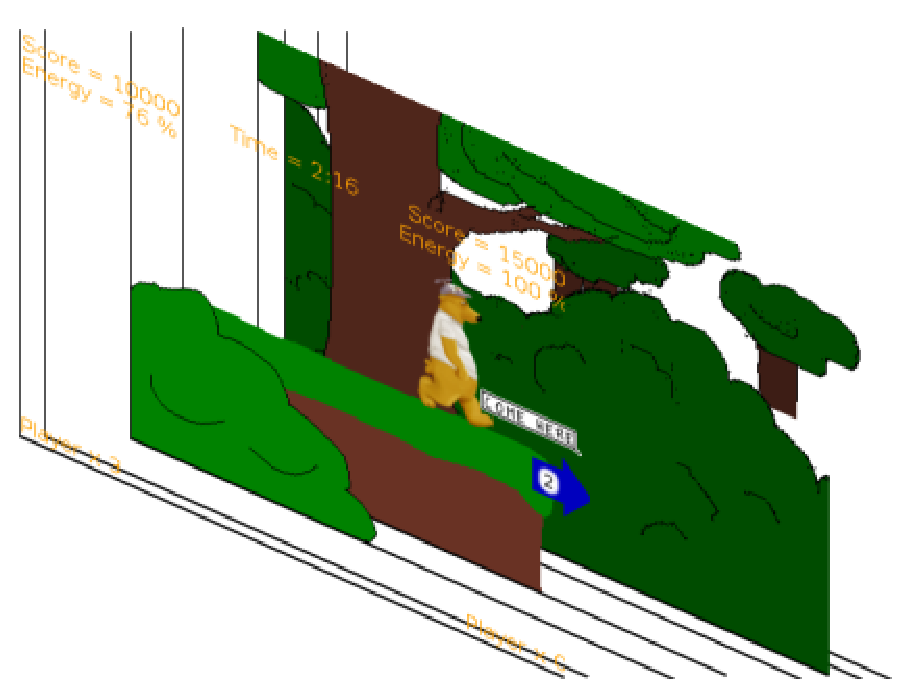
\includegraphics[width=9cm]{pictures/layers-separated}
  \caption{Les diff\'erents calques}
  \label{fig-layers-separated}
  \end{center}
\end{figure}

\begin{figure}
 \begin{center}
  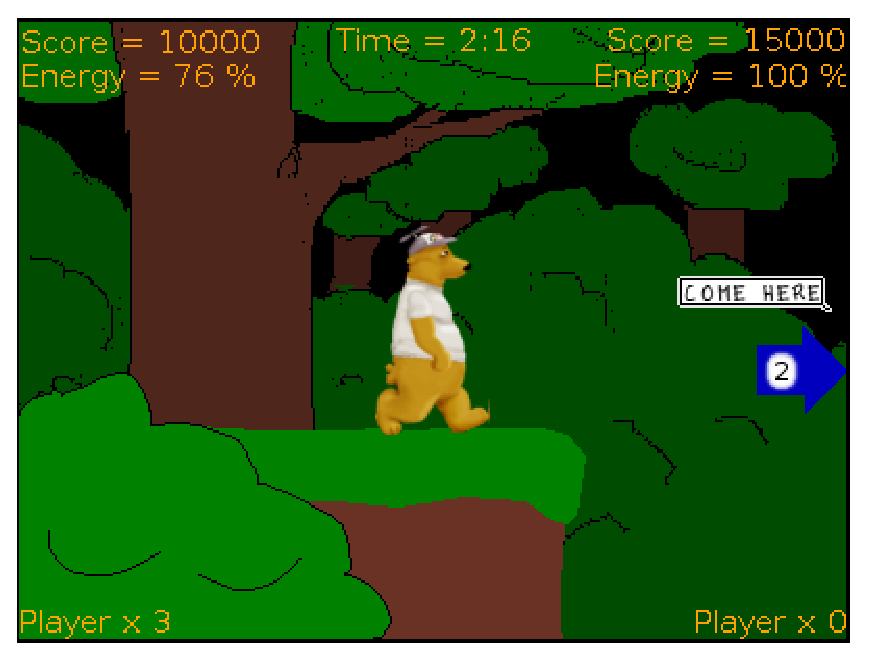
\includegraphics[width=9cm]{pictures/layers-result}
  \caption{La vue r\'esultante}
  \label{fig-layers-result}
 \end{center}
\end{figure}

\section{Restrictions sur les sprites}
Pour donner une id\'ee de l'\'echelle des sprites, la hauteur du
joueur est un tiers de la hauteur de l'\'ecran. La plupart du temps,
il sera plac\'e au milieu de l'\'ecran.

Le jeu ne fait pas de collisions au pixel pr\`es. Les objets sont
consid\'er\'es comme des rectangles, ils sont en collision si leurs
rectangles se coupent. Par exemple, si votre sprite est une ligne
de 14 pixels avec un angle de 45 degr\'es, il sera consid\'er\'e comme
un carr\'e de 10 pixels de cot\'e. Si deux de ces bo\^ites se coupent
en un seul pixel, il y aura collision ; m\^eme si les lignes semblent
\^etre loin l'une de l'autre. Nous autorisons que les bo\^ites aient
une taille diff\'erente de celle des sprites, comme �a on peut faire
des compromis.

Prenons le cercle vert de l'image~\ref{fig-bounding-box} en
exemple. Chaque bo\^ite entre les carr\'es rouges est candidate pour
\^etre la bo\^ite du sprite. Nous choisirons probablement la bo\^ite
interm\'ediaire. Bien que les objets se r\'eduisent \`a des
rectangles, essayez de faire des images avec des courbes. Les niveaux
ne doivent pas ressembler \`a un tas de pi\`eces carr\'ees mises cote
\`a cote.

\begin{figure}
\begin{center}
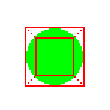
\includegraphics{pictures/bounding-box}
\caption{Bo\^ites englobantes pour un cercle.}
\label{fig-bounding-box}
\end{center}
\end{figure}

\section{Comment faire de beaux dessins}

Le jeu ressemblera \`a une belle image soigneusement dessin\'ee ;
quelque chose entre le dessin plat fait par un enfant et l'image
froide que peut faire un logiciel de mod\'elisation 3D. Vous devez
penser <<~(jolie) bande dessin\'ee~>> :

\begin{itemize}
\item on doit voir que les images sont faites � la main ;
\item on ne devrait jamais voir deux fois le m\^eme sprite de
      d\'ecoration \`a l'\'ecran ;
\item les images doivent \^etre aussi d\'etaill\'ees que possible.
\end{itemize}

\begin{figure}
   \begin{minipage}[c]{.46\linewidth}
     \begin{center}
      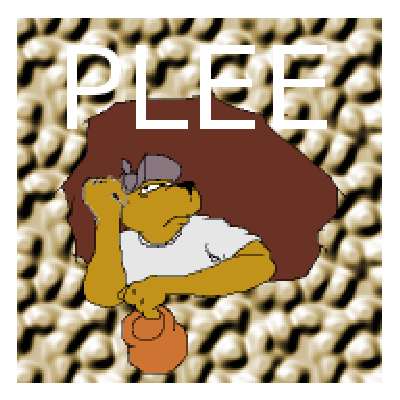
\includegraphics[width=5.5cm]{pictures/bad}
      \caption{Mauvais dessin}
      \label{fig-bad}
     \end{center}
   \end{minipage} \hfill
   \begin{minipage}[c]{.46\linewidth}
     \begin{center}
      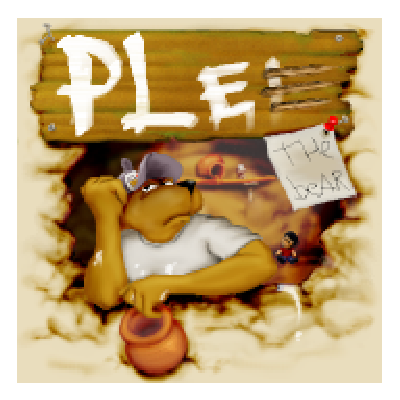
\includegraphics[width=5.5cm]{pictures/good}
      \caption{Bon dessin}
      \label{fig-good}
     \end{center}
   \end{minipage}
\end{figure}

Prenons les images \ref{fig-bad} et \ref{fig-good} comme
exemples. Pour la premi\`ere, m\^eme si on peut voir et comprendre que
Plee est l\`a avec un pot de miel dans sa main, personne ne voudrais
regarder cette image plus d'une seconde. Alors que la seconde image
est plus d\'etaill\'ee, on voudrait trouver tous les d\'etails, depuis
les petits clous jusqu'aux marques de peinture sur les bras de Plee.

\'Evitez les textures r\'ep\'etitives et \'evitez toute image fournie
avec votre logiciel de dessin. Le joueur doit penser <<~Waow ! C'est
un unique et joli \'ecran !~>>, pas <<~Hey ! Ils ont prit \c ca dans
photoshop !~>>.

La r\`egle finale sera : <<~si c'est suffisant pour vous, essayez de faire
mieux~>>.


\end{document}
